\documentclass[10pt]{beamer}
\usepackage[utf8]{inputenc}
\usetheme{metropolis}
\usecolortheme{beaver}
\title{Časovne vrste - seminarska naloga}
\author{\centering Brina Pirc in Anja Trobec}
\vspace{3pt}
\institute{\centering Fakulteta za Matematiko in Fiziko}
\date{\centering Maj, 2022}

\begin{document}

\frame{\titlepage}

\begin{frame}
\frametitle{Časovna vrsta A}
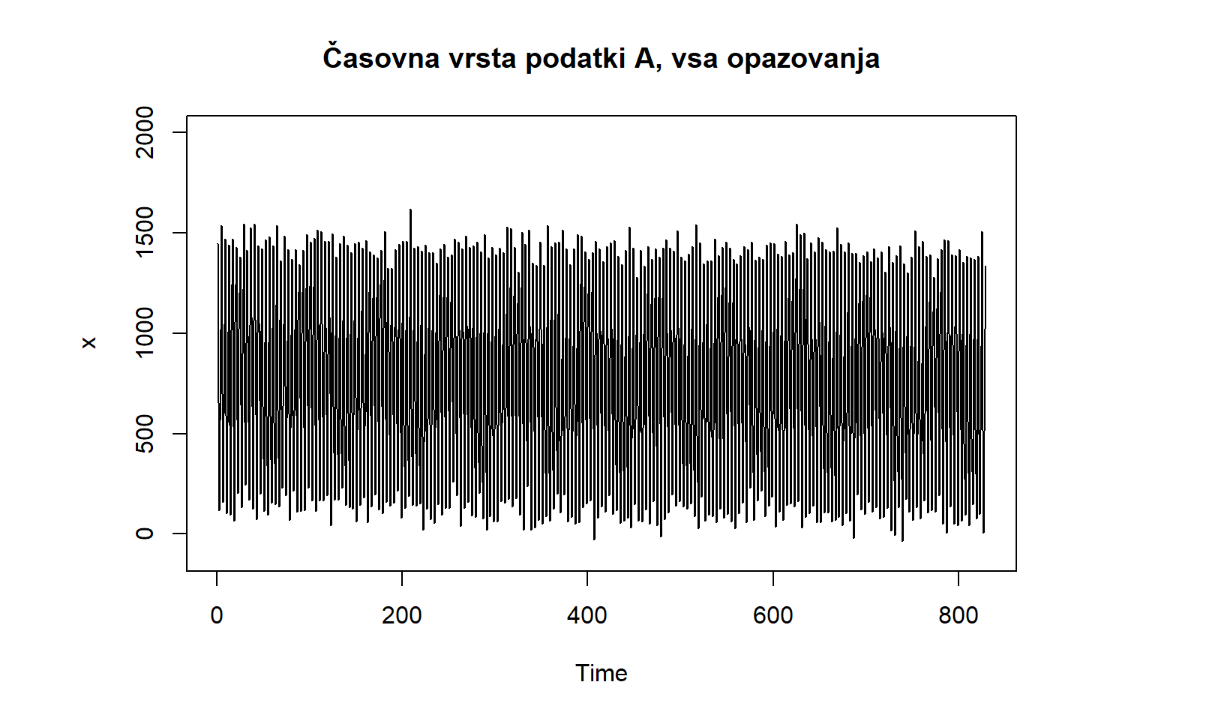
\includegraphics[width=1\textwidth]{casovnaA.png}
\end{frame}


\begin{frame}
\frametitle{Časovna vrsta A - 100 opazovanj}
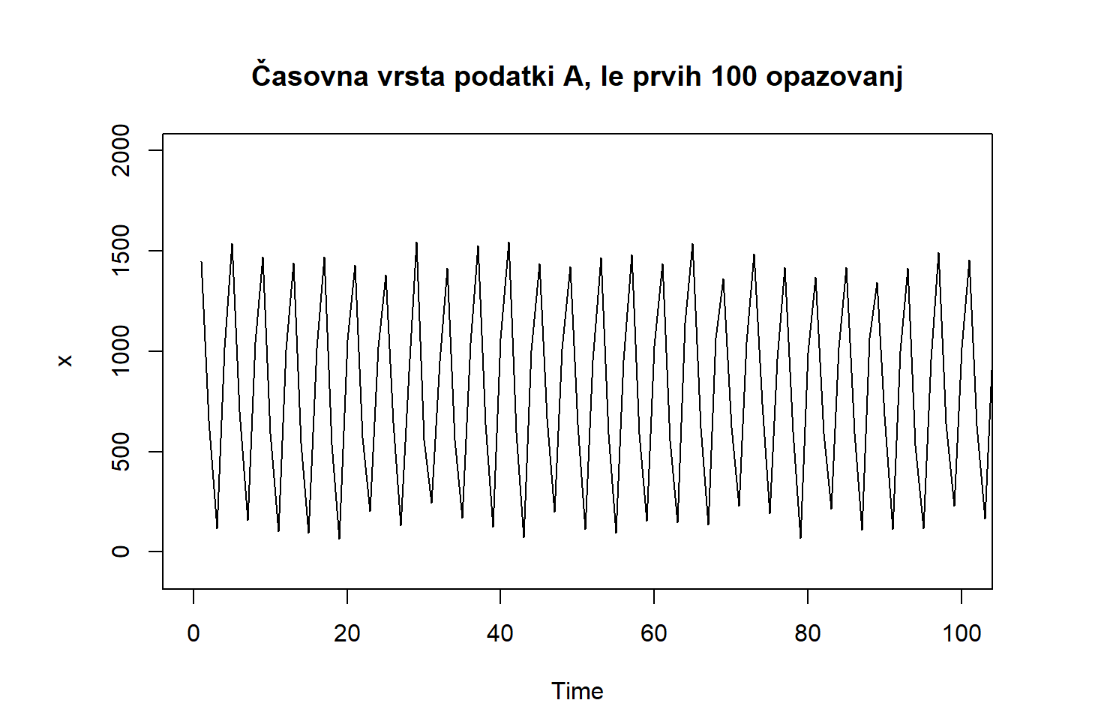
\includegraphics[width=1\textwidth]{casovnaA100.png}
\end{frame}

\begin{frame}
\frametitle{Diference}
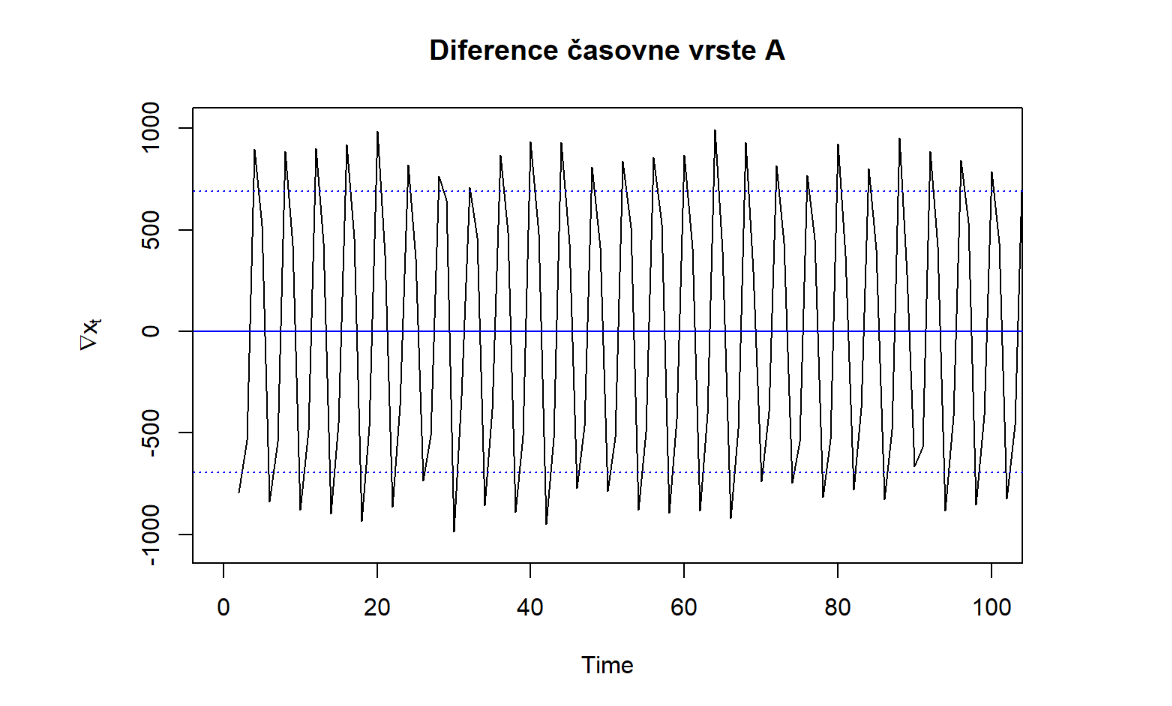
\includegraphics[width=1\textwidth]{diff_A.png}
\end{frame}

\begin{frame}
\frametitle{Trend in sezonskost - dekompozicija}
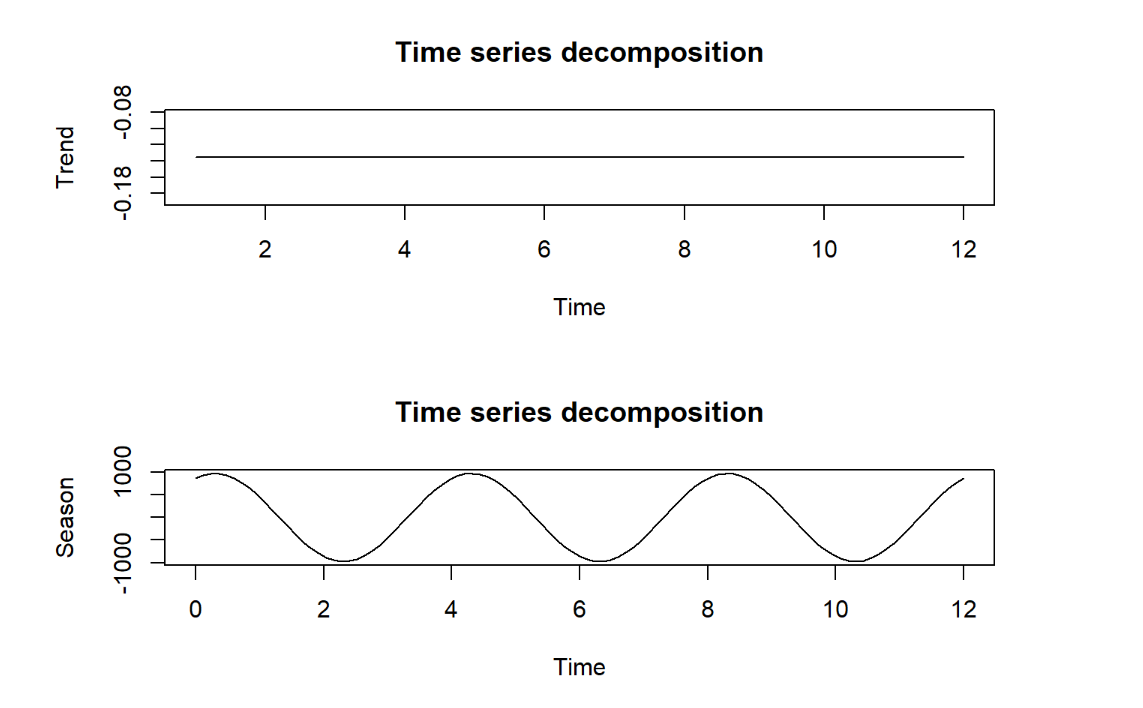
\includegraphics[width=1\textwidth]{decompositionA.png}
\end{frame}


\begin{frame}
\frametitle{Harmonična regresija}
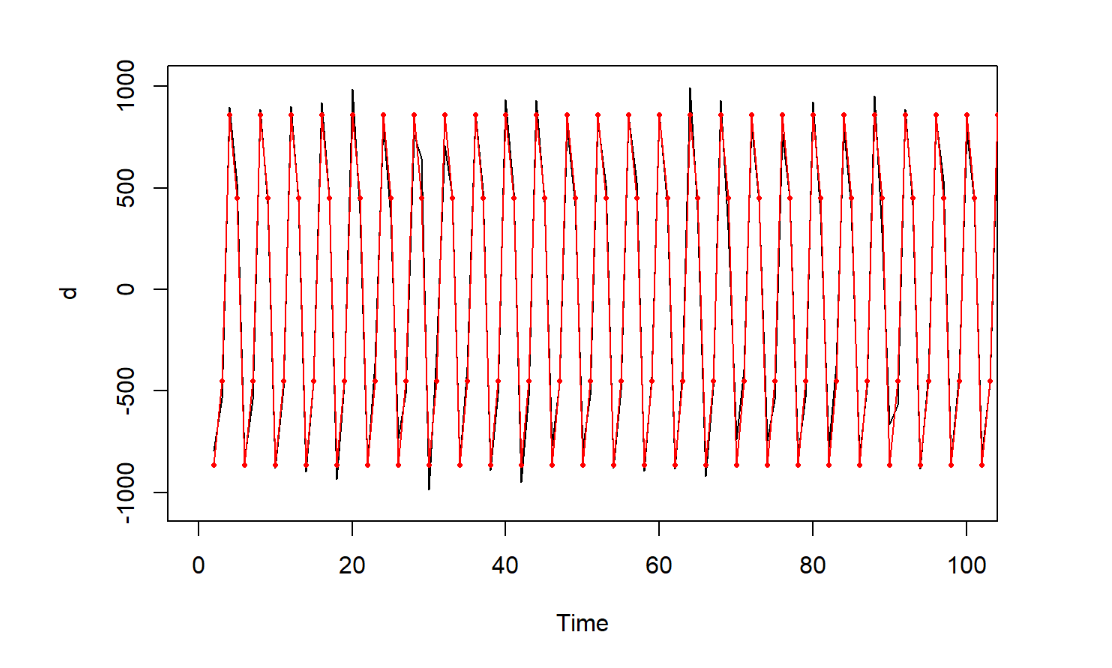
\includegraphics[width=1\textwidth]{fit_A.png}
\end{frame}

\begin{frame}
\frametitle{Surovi periodogram}
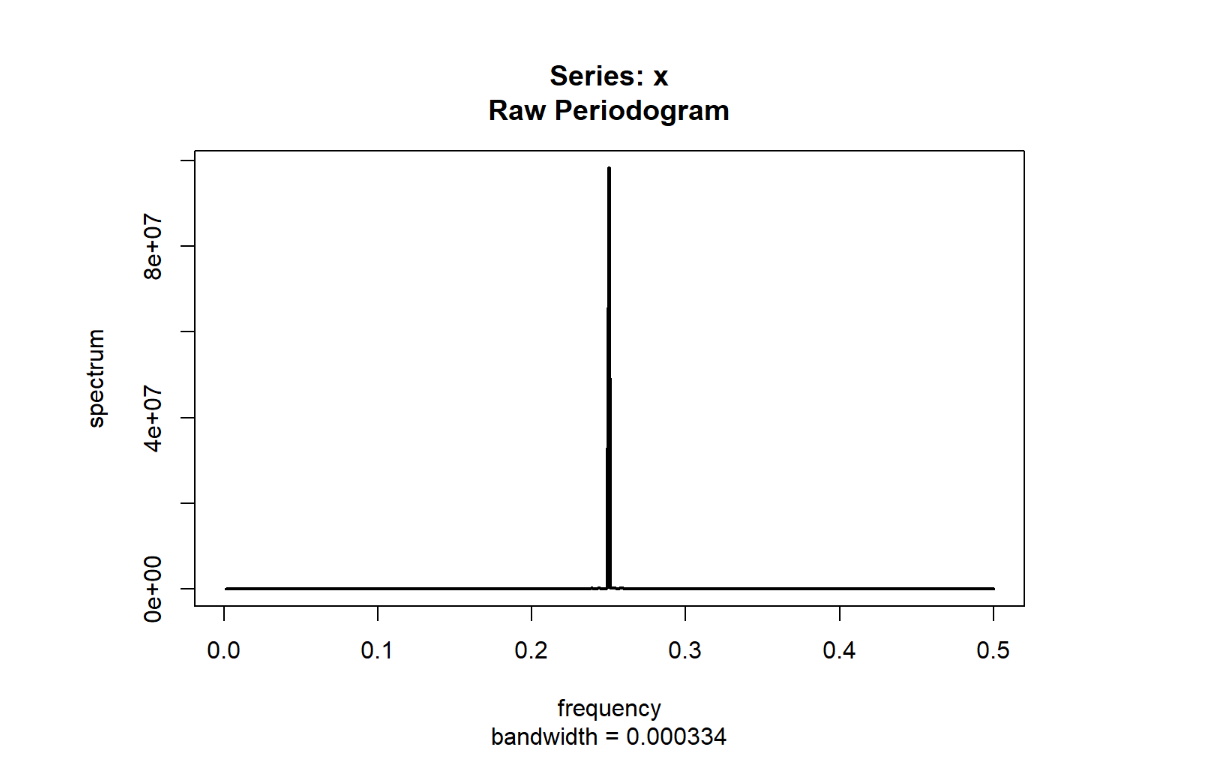
\includegraphics[width=1\textwidth]{per_raw1A.png}
\end{frame}

\begin{frame}
\frametitle{Zglajeni periodogram}
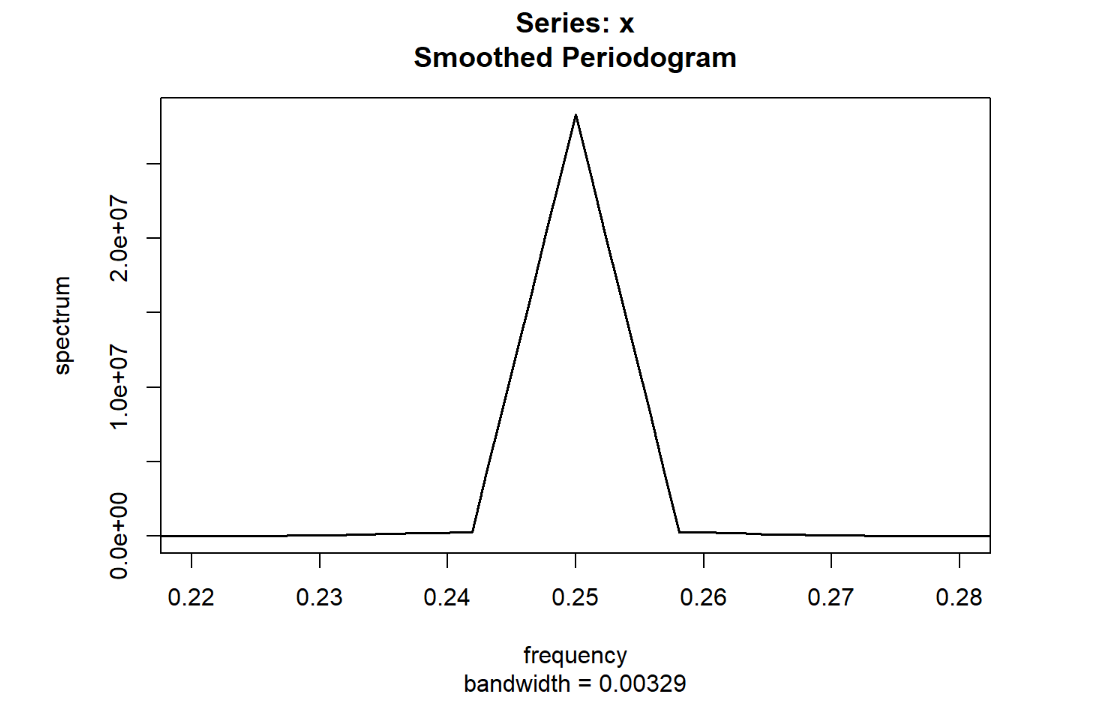
\includegraphics[width=1\textwidth]{per_raw2A.png}
\end{frame}

\begin{frame}
\frametitle{Residuali - stacionarnost}
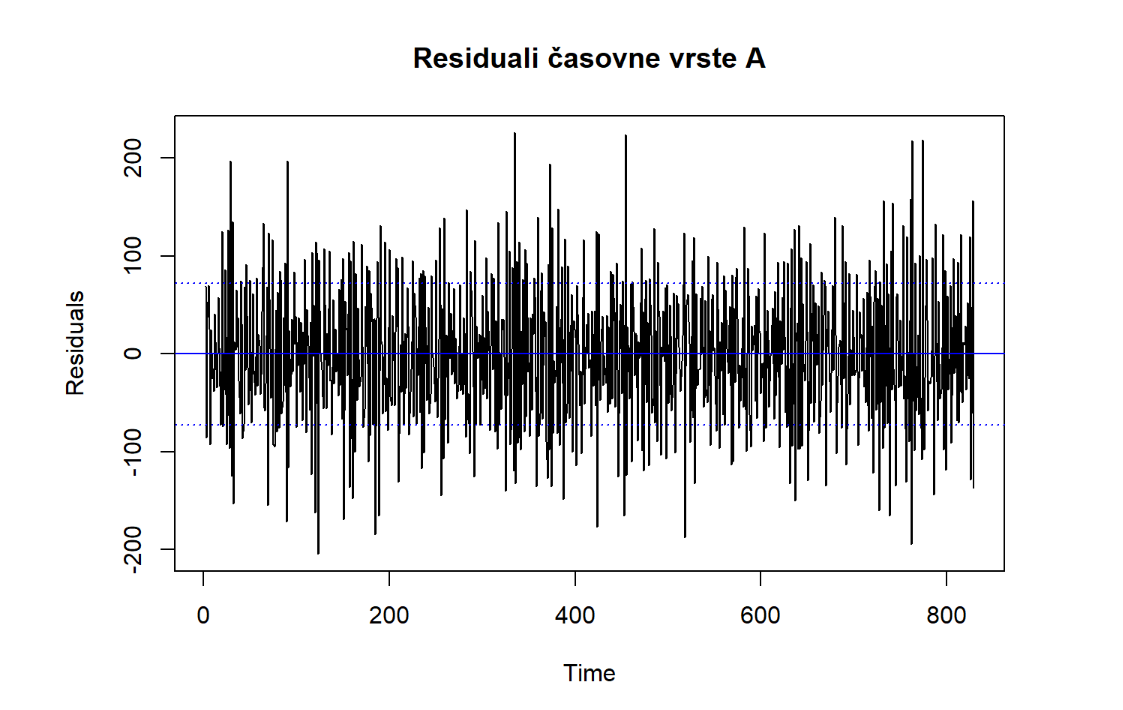
\includegraphics[width=1\textwidth]{res_casA.png}
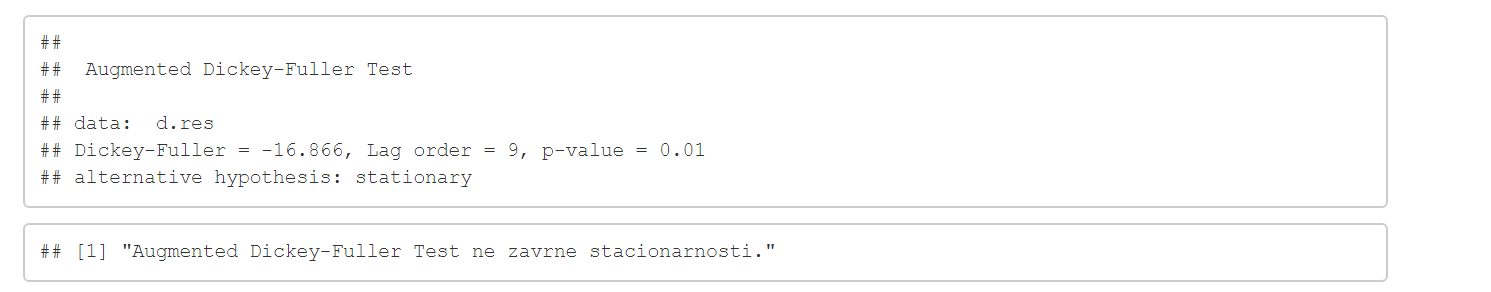
\includegraphics[width=1\textwidth]{DickyTestA.png}
Test ne zavrne stacionarnosti.
\end{frame}

\begin{frame}
\frametitle{ACF in predlog za model MA(p)}
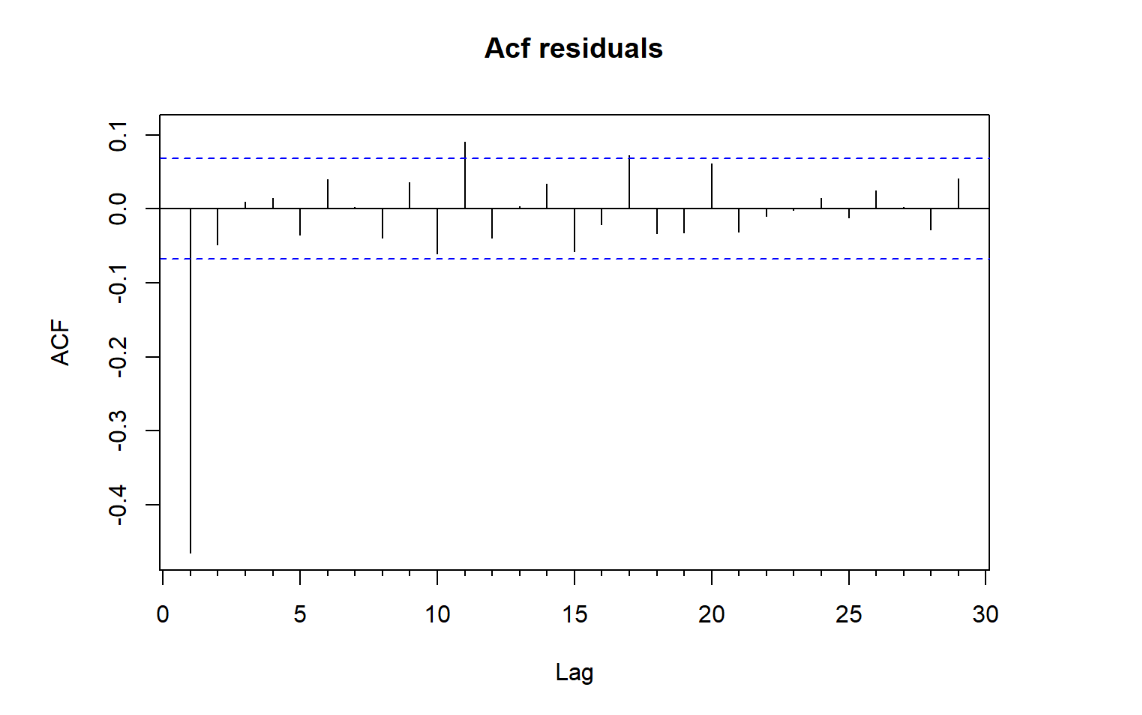
\includegraphics[width=1\textwidth]{AcfA.png}
\end{frame}

\begin{frame}
\frametitle{PACF in predlog za model AR(q)}
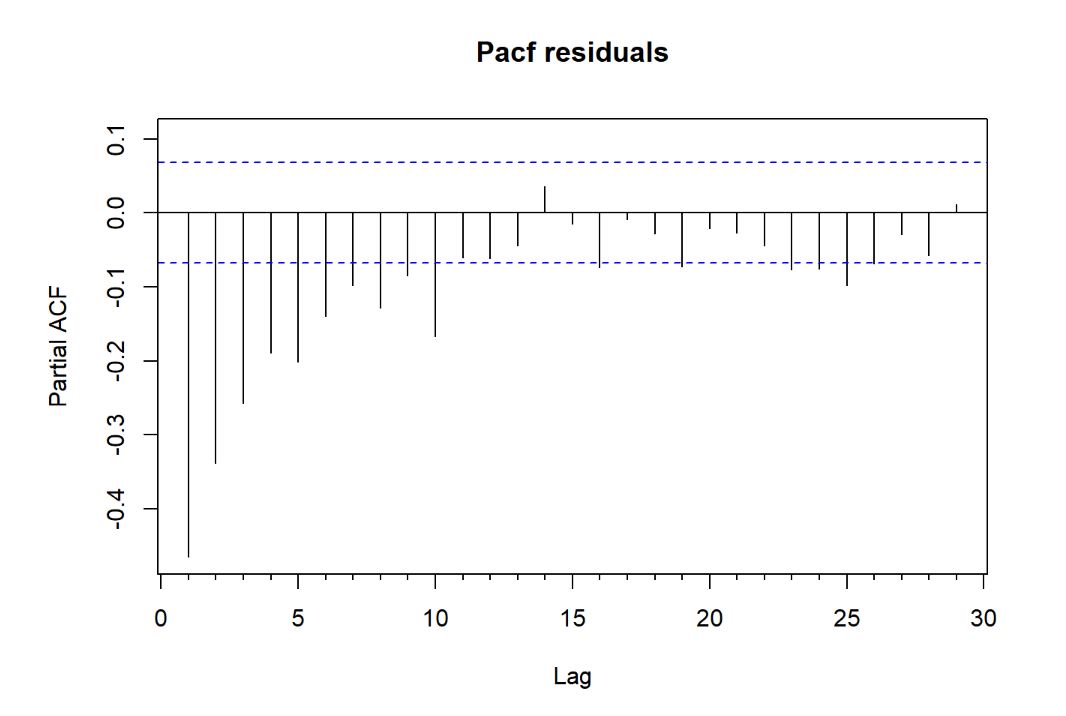
\includegraphics[width=1\textwidth]{PacfA.png}
\end{frame}

\begin{frame}
\frametitle{Izbira modela ARMA(p,q) za $ p + q \le 3$}
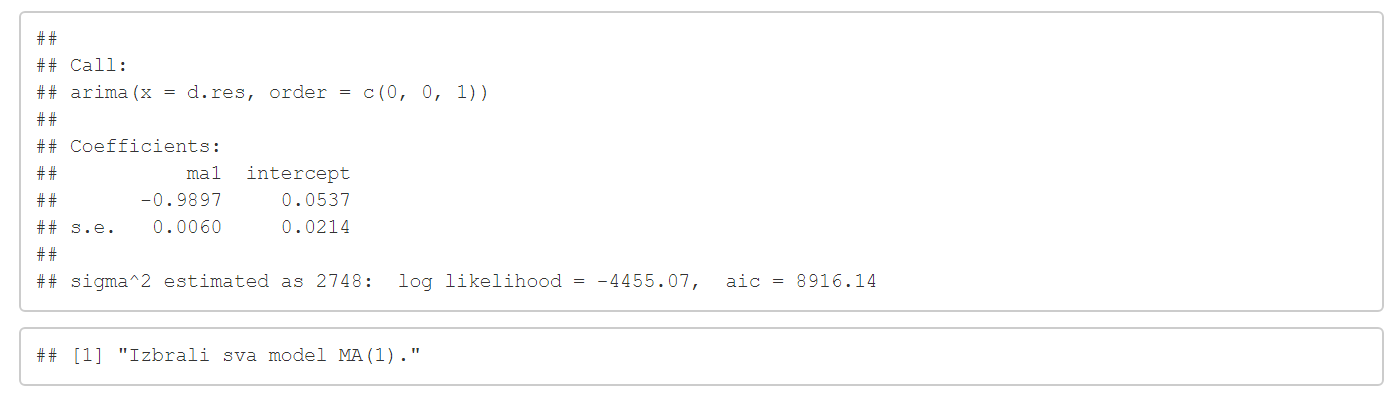
\includegraphics[width=1\textwidth]{ModelA.png}
\end{frame}


\begin{frame}
\frametitle{Test za normalno porazdelitev}
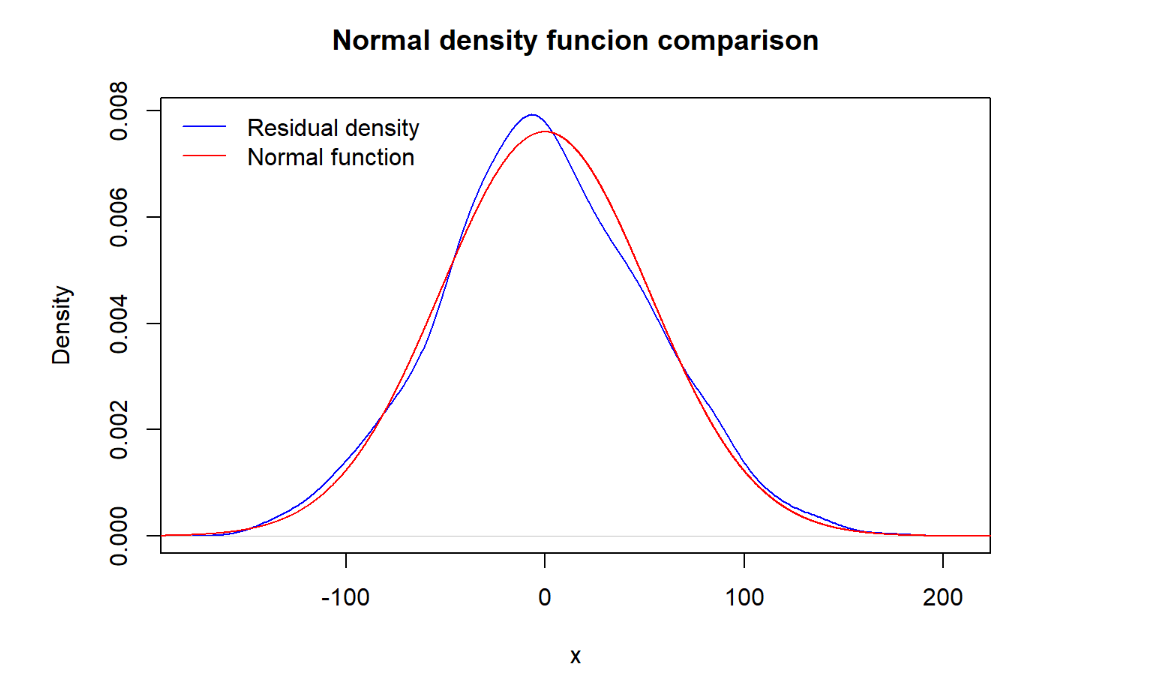
\includegraphics[width=1\textwidth]{normalnaA.png}

\end{frame}

\begin{frame}
\frametitle{Test za normalno porazdelitev}
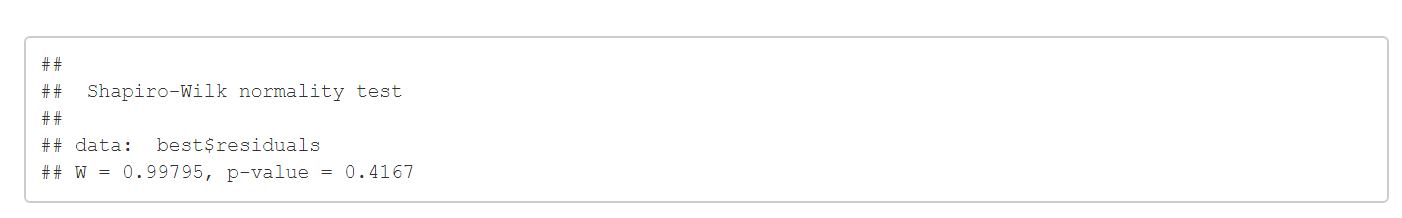
\includegraphics[width=1\textwidth]{ShapiroA.png}

\end{frame}


\begin{frame}
\frametitle{White Noise}
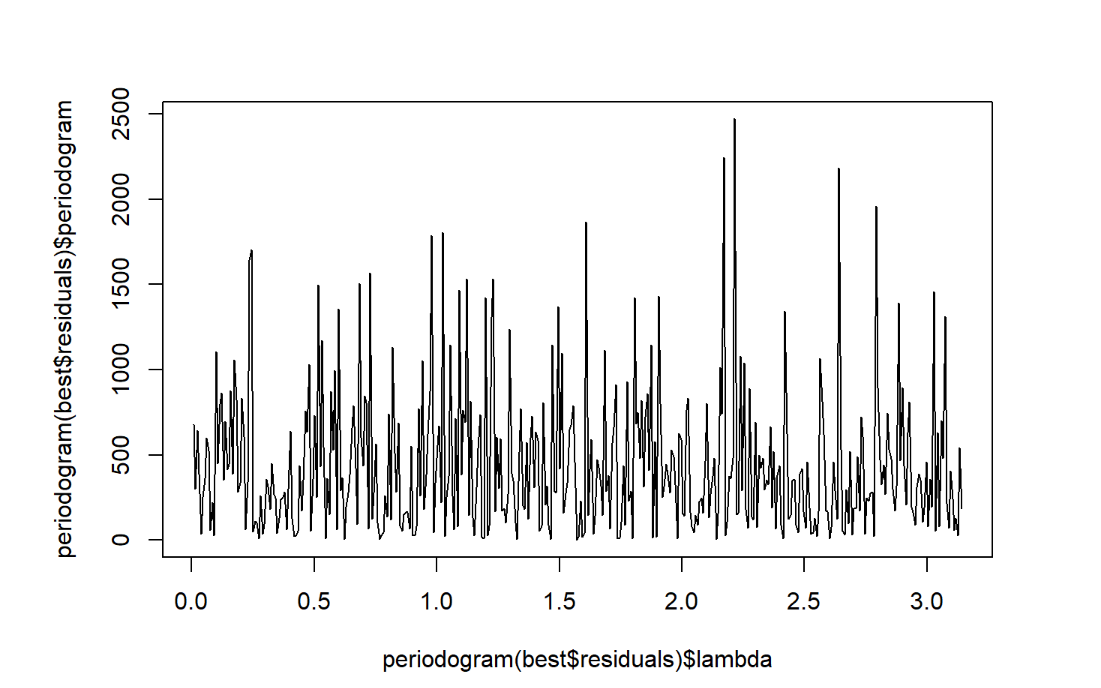
\includegraphics[width=1\textwidth]{whiteA.png}
\end{frame}

\begin{frame}
\frametitle{White Noise}
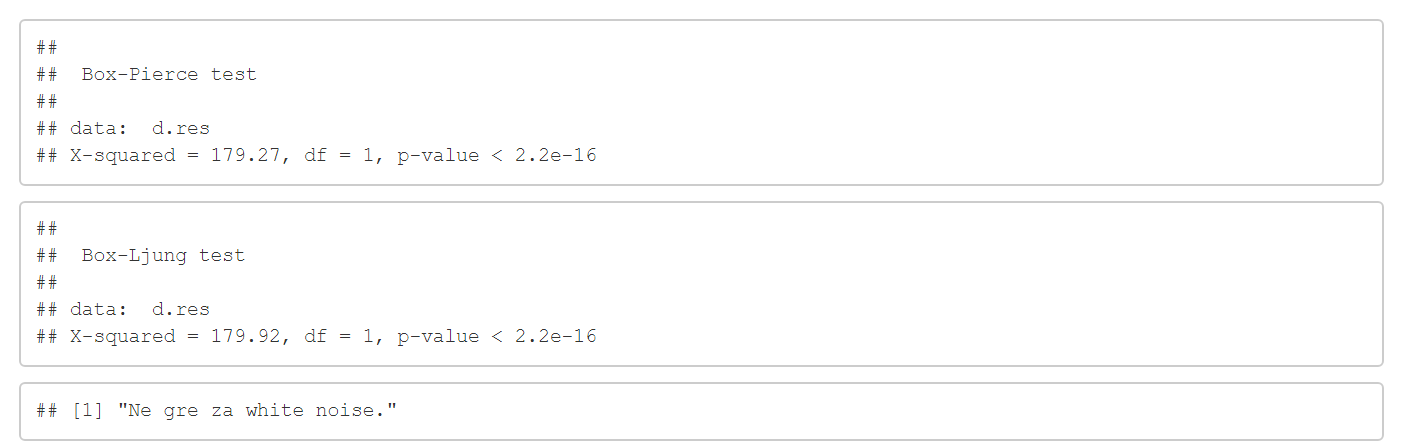
\includegraphics[width=1\textwidth]{testwnA.png}
\end{frame}



\begin{frame}
\frametitle{Napoved časovne vrste A}
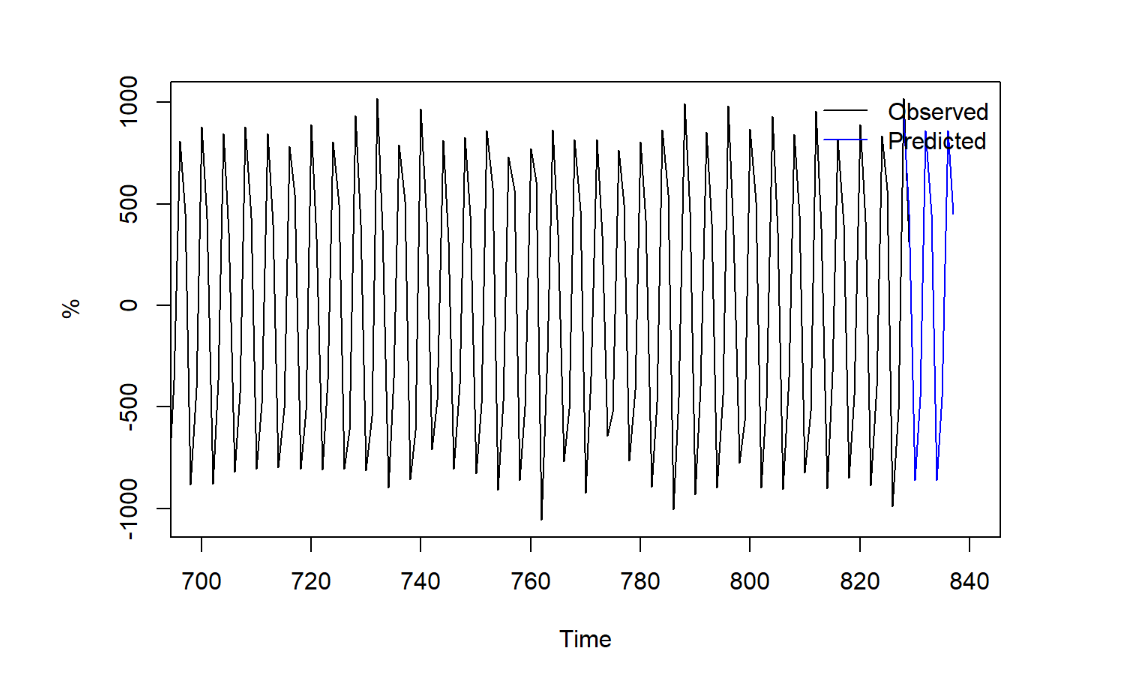
\includegraphics[width=1\textwidth]{predA.png}
\end{frame}


\begin{frame}
\frametitle{Gaussova napoved}
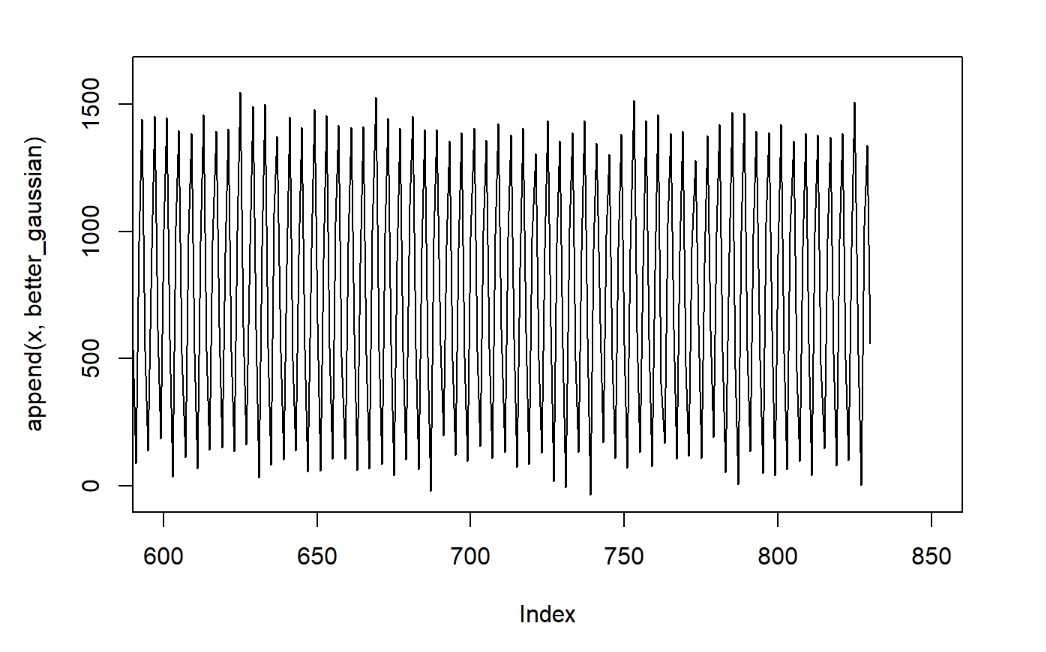
\includegraphics[width=1\textwidth]{betterA.png}
\end{frame}
\begin{frame}
\frametitle{Gaussova napoved}
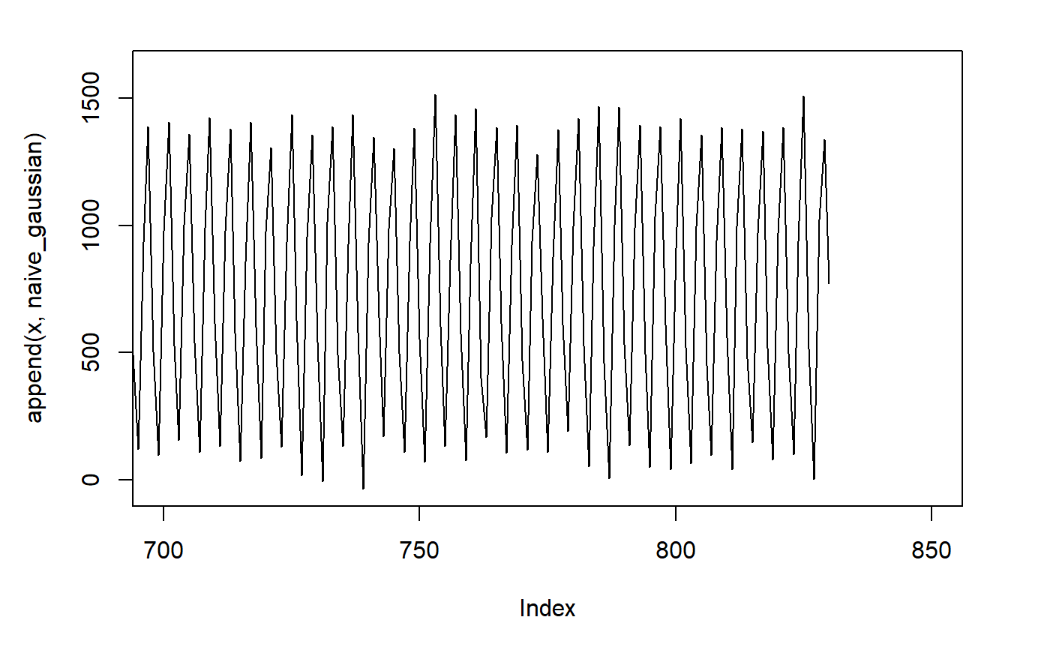
\includegraphics[width=1\textwidth]{naiveA.png}
\end{frame}
\begin{frame}
\frametitle{Gaussova napoved}
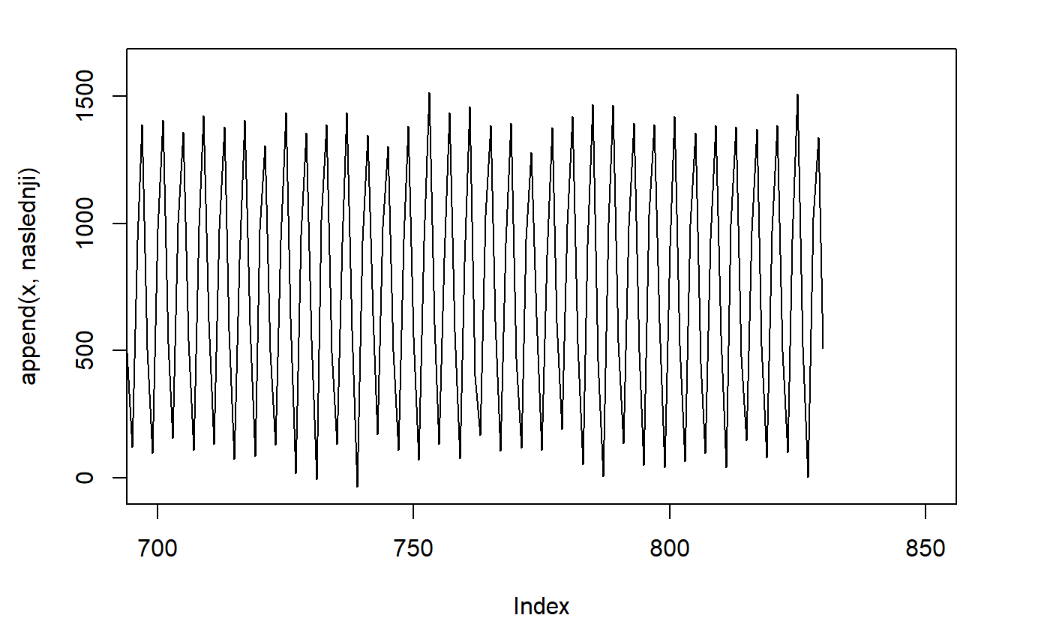
\includegraphics[width=1\textwidth]{naslednjiA.png}
\end{frame}

%___________________________________________________________________________________________

\begin{frame}
\frametitle{Časovna vrsta B}

\end{frame}



\begin{frame}
\frametitle{Časovna vrsta B}
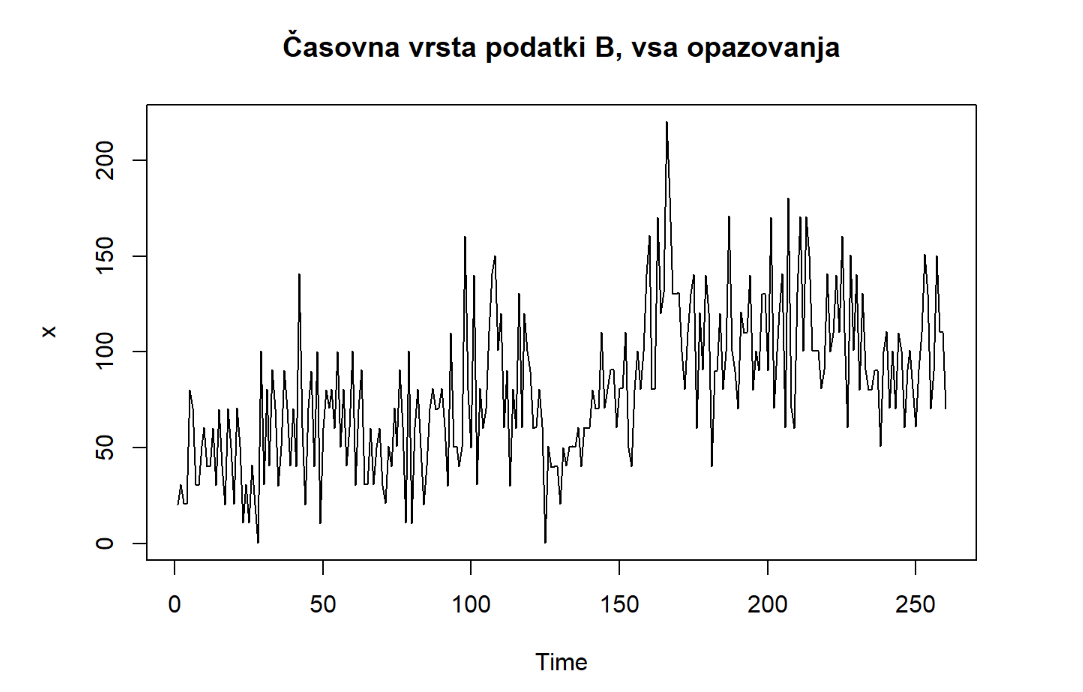
\includegraphics[width=1\textwidth]{casovnaB.png}
\end{frame}

\begin{frame}
\frametitle{Logaritmirana časovna vrsta B}
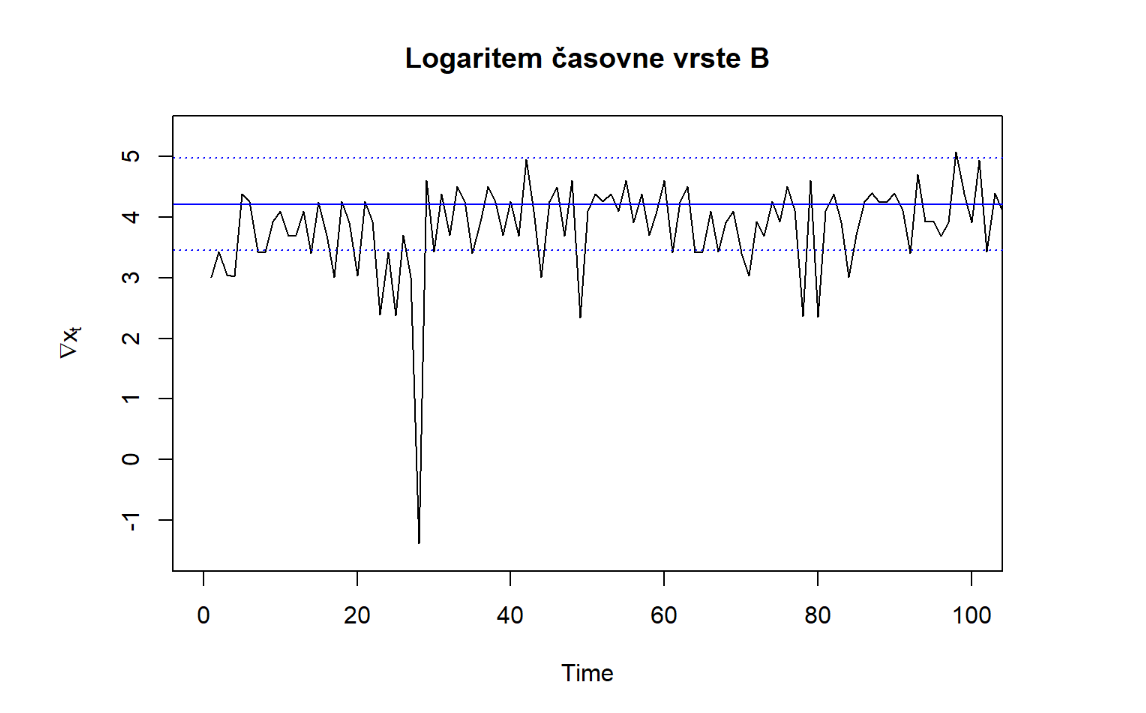
\includegraphics[width=1\textwidth]{logB.png}
\end{frame}


\begin{frame}
\frametitle{Harmonična regresija}
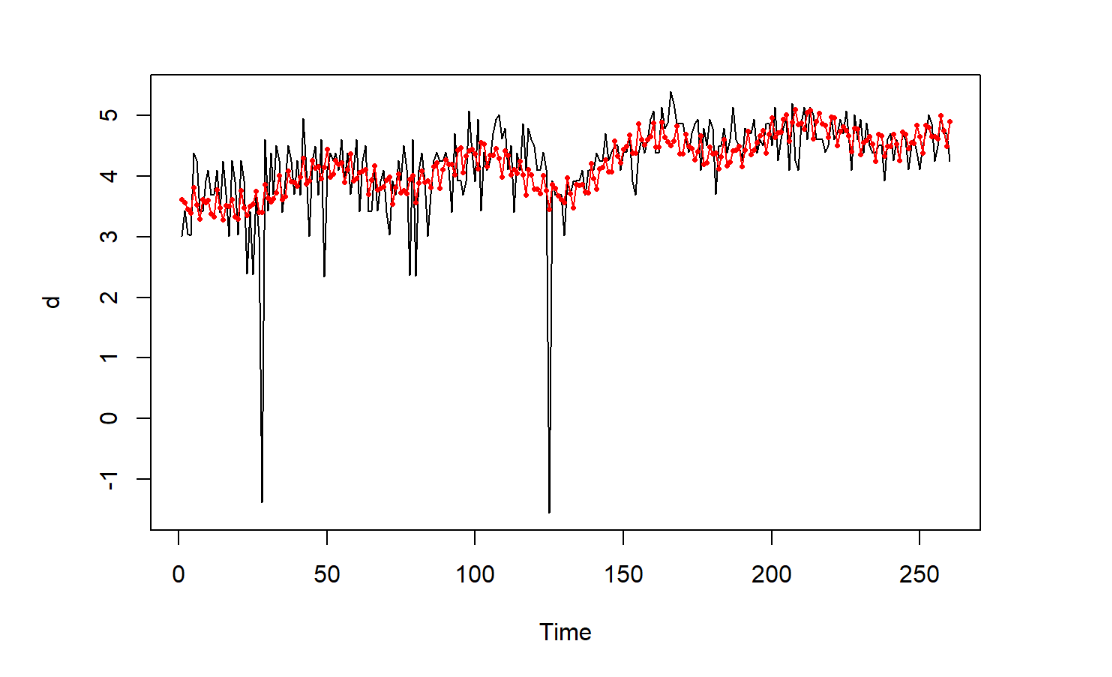
\includegraphics[width=1\textwidth]{fitB.png}
\end{frame}

\begin{frame}
\frametitle{Trend in sezonskost - dekompozicija}
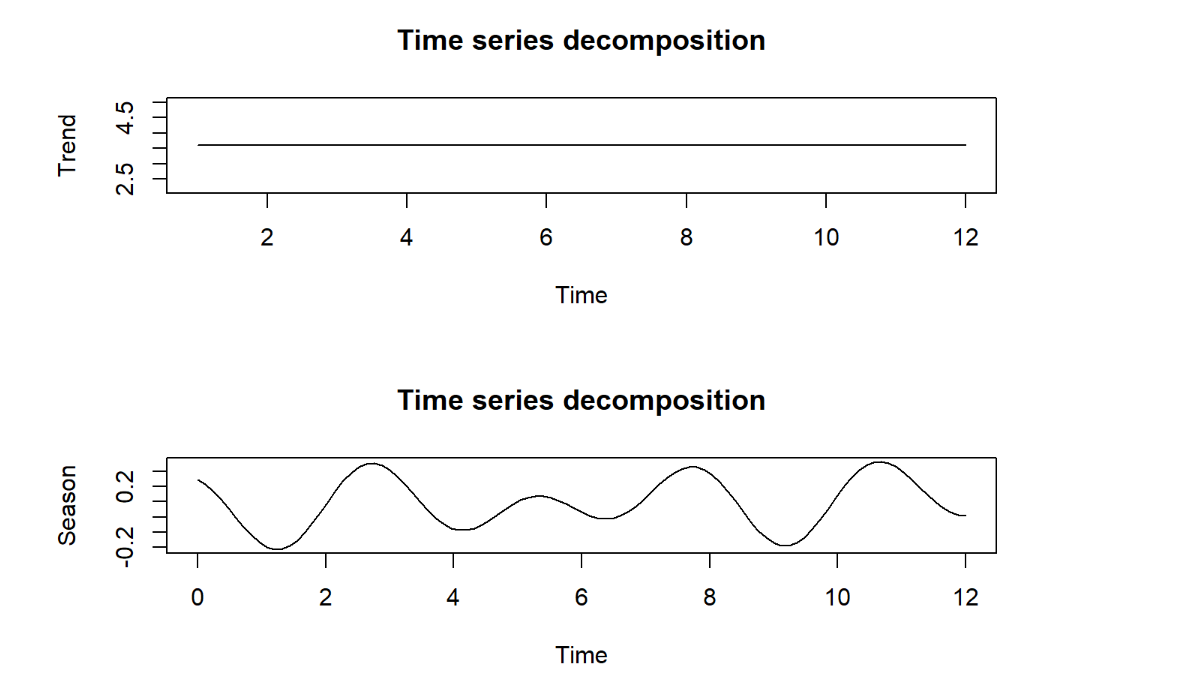
\includegraphics[width=1\textwidth]{seasonB.png}
\end{frame}

\begin{frame}
\frametitle{Residuali - stacionarnost}
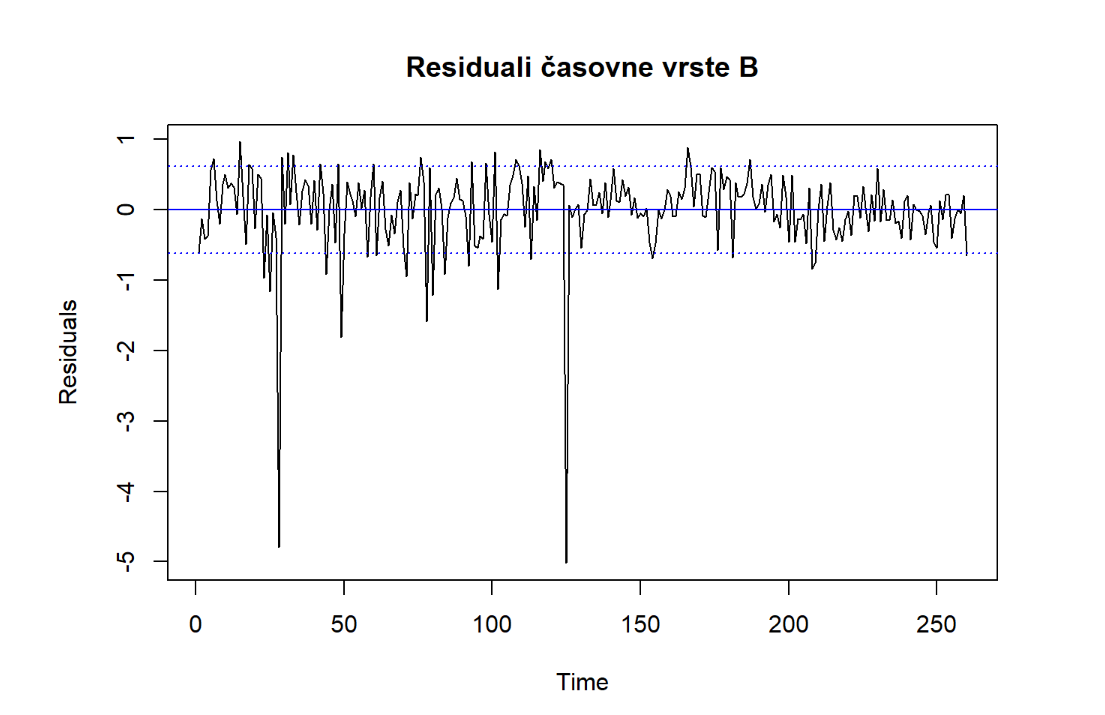
\includegraphics[width=1\textwidth]{res_log_B.png}
\end{frame}

\begin{frame}
\frametitle{Residuali - stacionarnost}
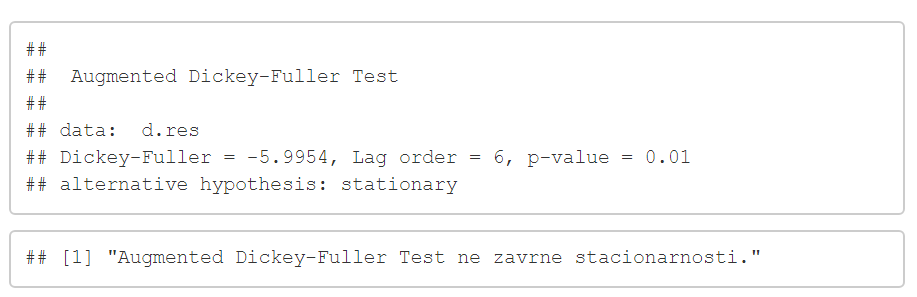
\includegraphics[width=1\textwidth]{stacionarnostB.png}
\end{frame}


\begin{frame}
\frametitle{ACF}
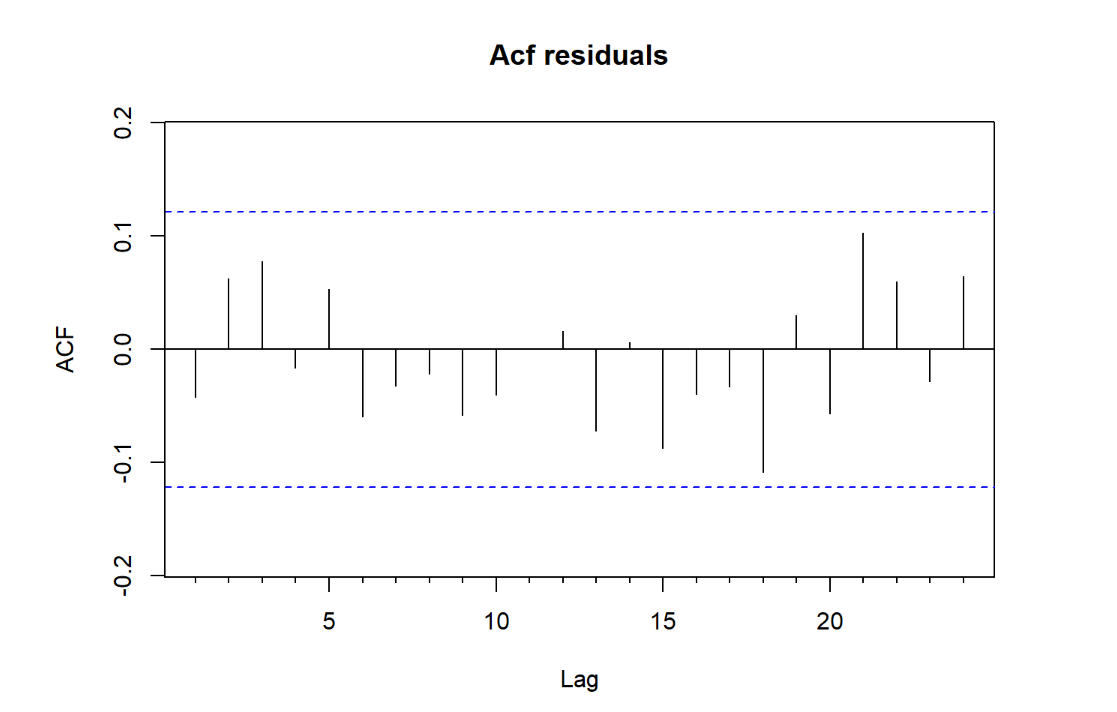
\includegraphics[width=1\textwidth]{AcfB.png}
\end{frame}

\begin{frame}
\frametitle{PACF}
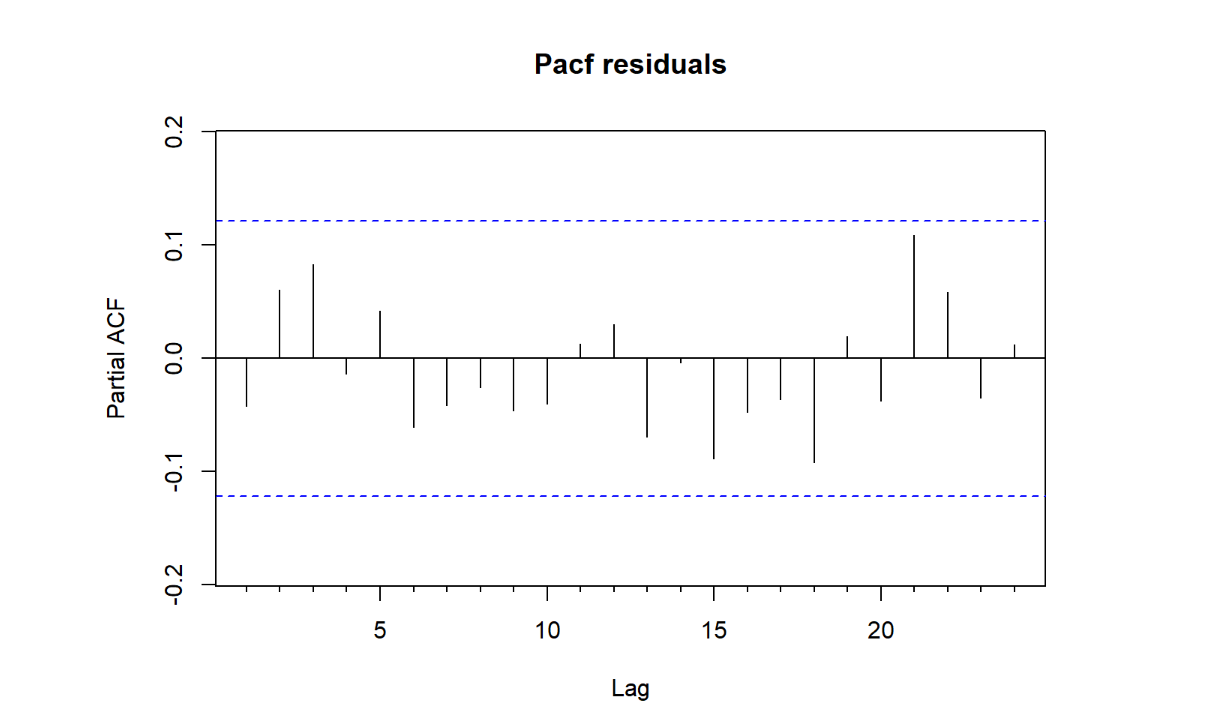
\includegraphics[width=1\textwidth]{PacfB.png}
\end{frame}


\begin{frame}
\frametitle{Residuali}
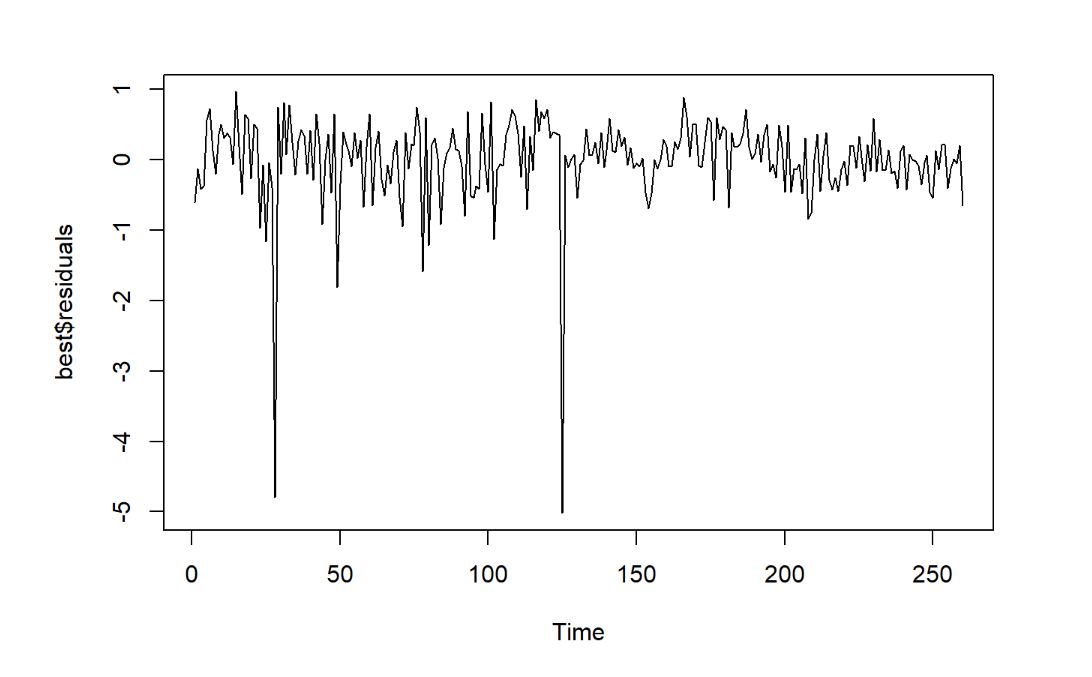
\includegraphics[width=1\textwidth]{best_res_B.png}
\end{frame}



\begin{frame}
\frametitle{Izbira modela}
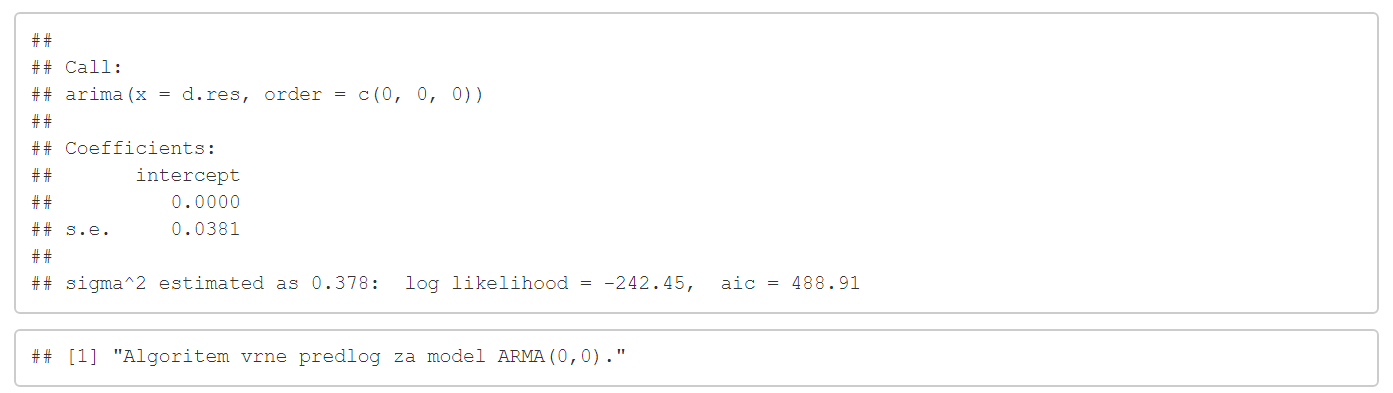
\includegraphics[width=1\textwidth]{ModelB.png}
\end{frame}


\begin{frame}
\frametitle{Test za normalno porazdelitev}
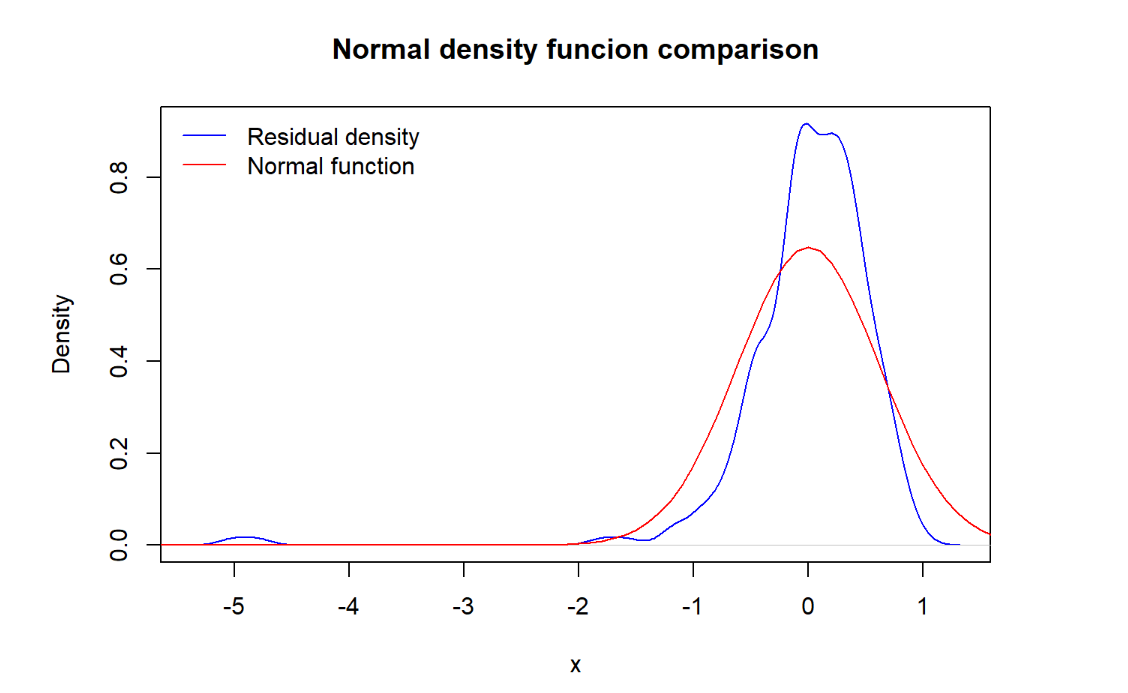
\includegraphics[width=1\textwidth]{normalnaB.png}

\end{frame}

\begin{frame}
\frametitle{Test za normalno porazdelitev}
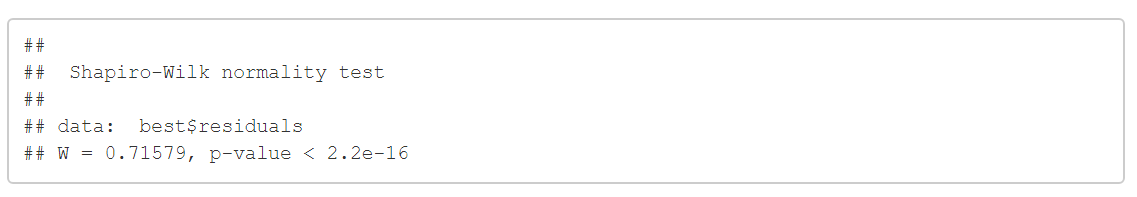
\includegraphics[width=1\textwidth]{ShapiroB.png}
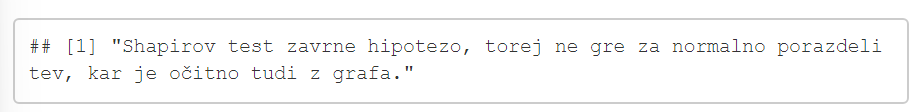
\includegraphics[width=1\textwidth]{ninormalnaB.png}

\end{frame}

\begin{frame}
\frametitle{White Noise}
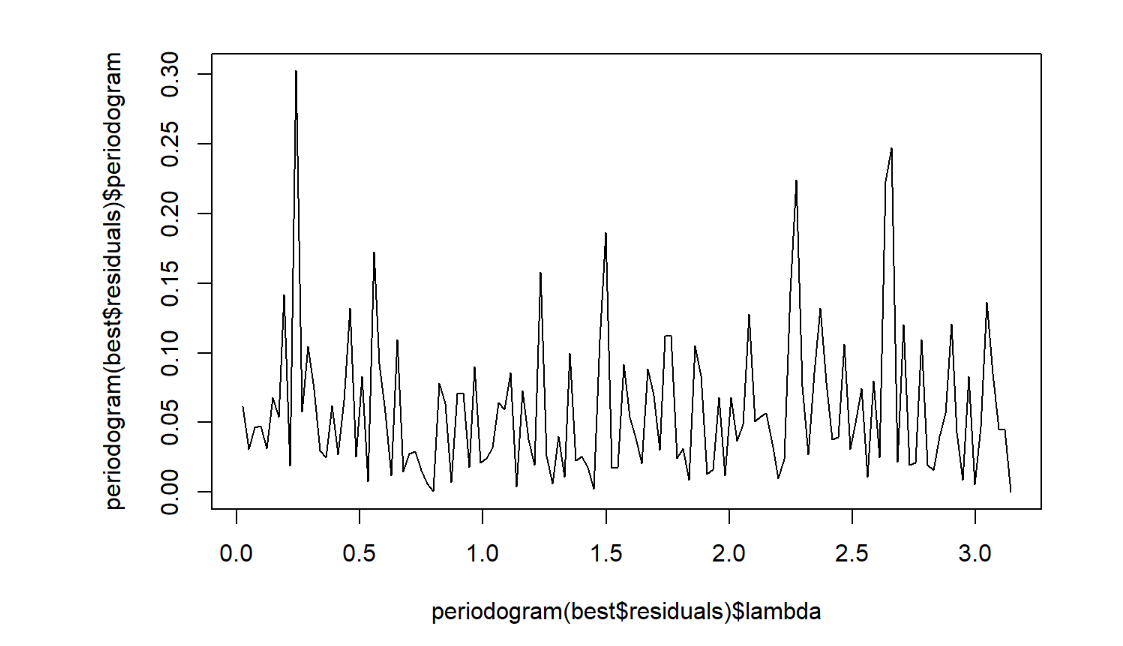
\includegraphics[width=1\textwidth]{white_noiseB.png}
\end{frame}

\begin{frame}
\frametitle{White Noise}
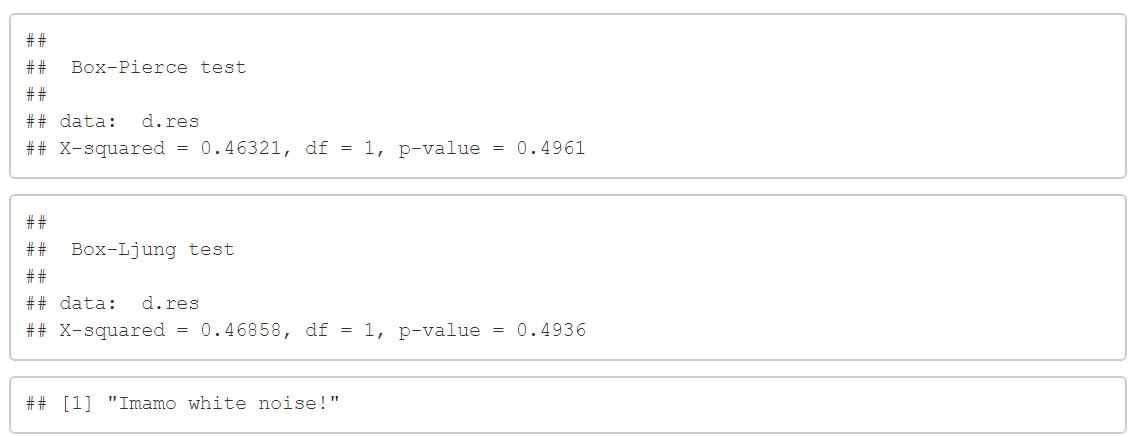
\includegraphics[width=1\textwidth]{testwnB.png}
\end{frame}



\begin{frame}
\frametitle{Napoved časovne vrste B}
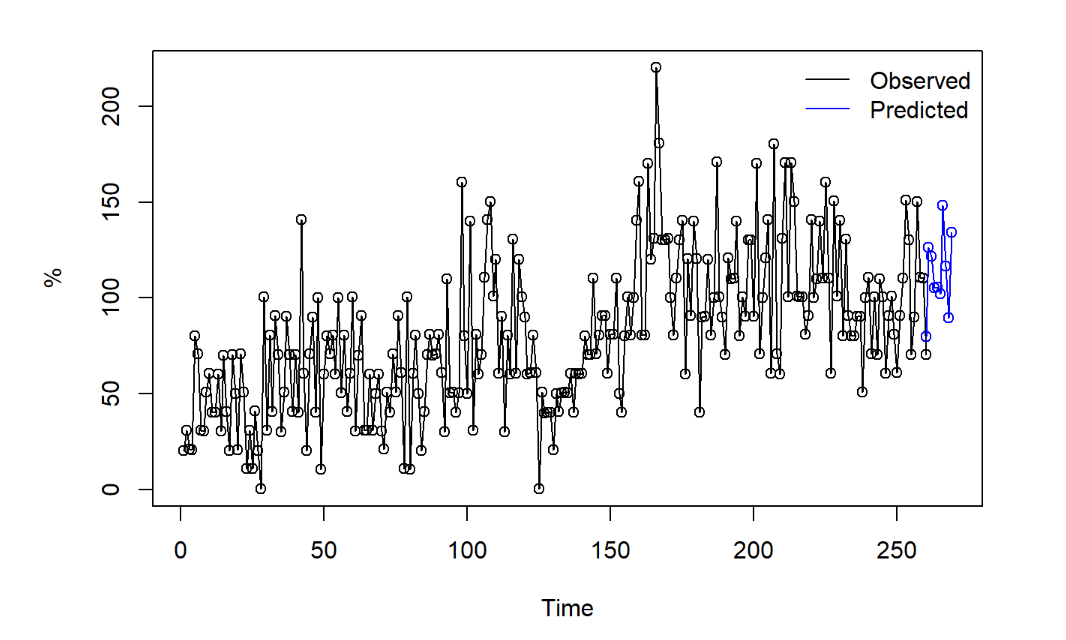
\includegraphics[width=1\textwidth]{napovedB.png}
\end{frame}


\begin{frame}
\frametitle{Gaussova napoved}
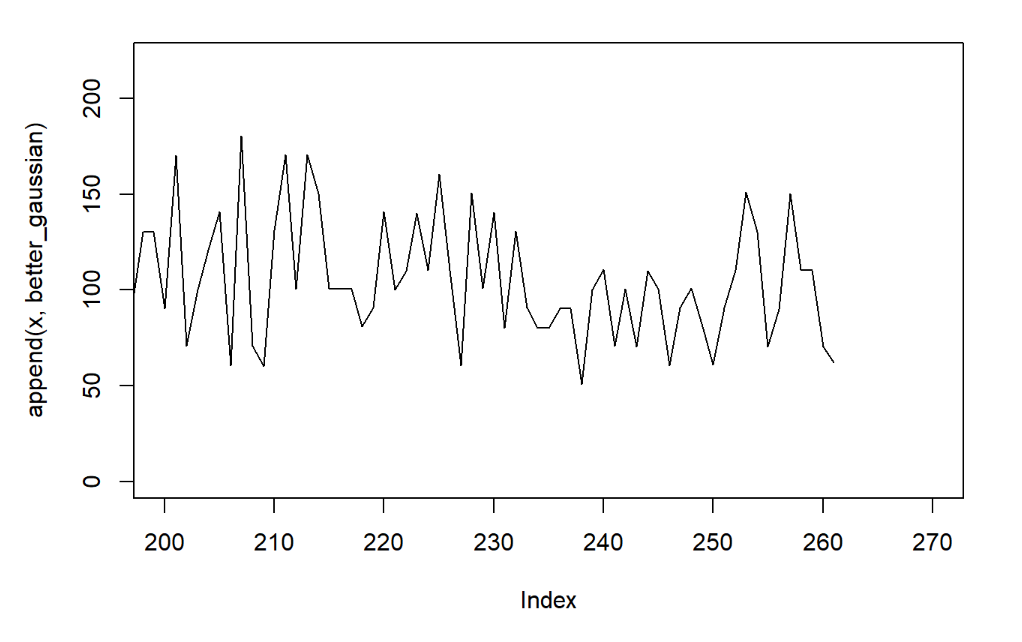
\includegraphics[width=1\textwidth]{betterB.png}
\end{frame}
\begin{frame}
\frametitle{Gaussova napoved}
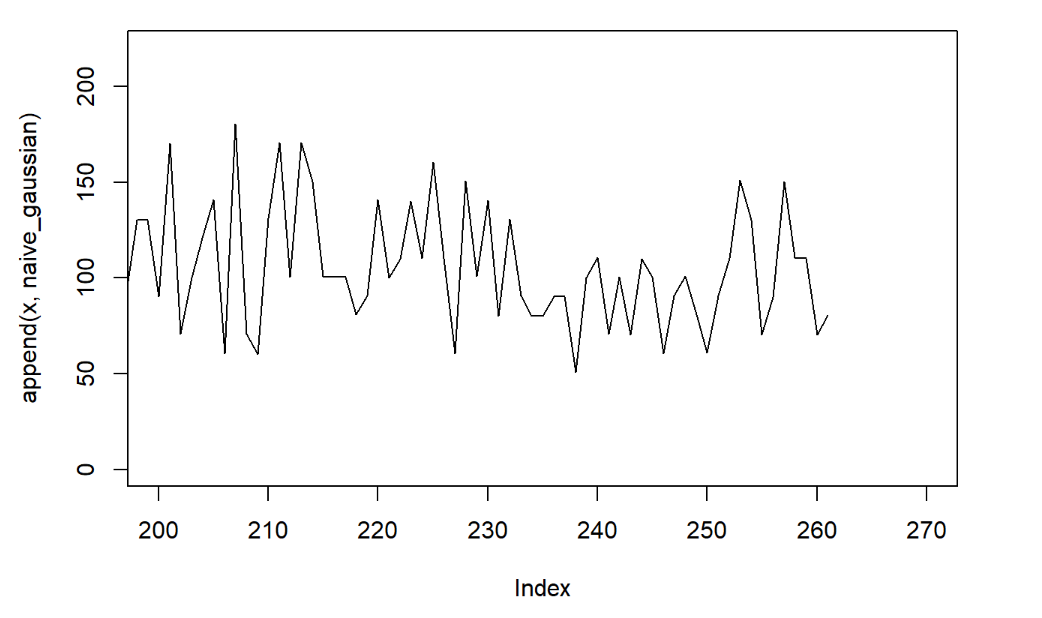
\includegraphics[width=1\textwidth]{naiveB.png}
\end{frame}
\begin{frame}
\frametitle{Gaussova napoved}
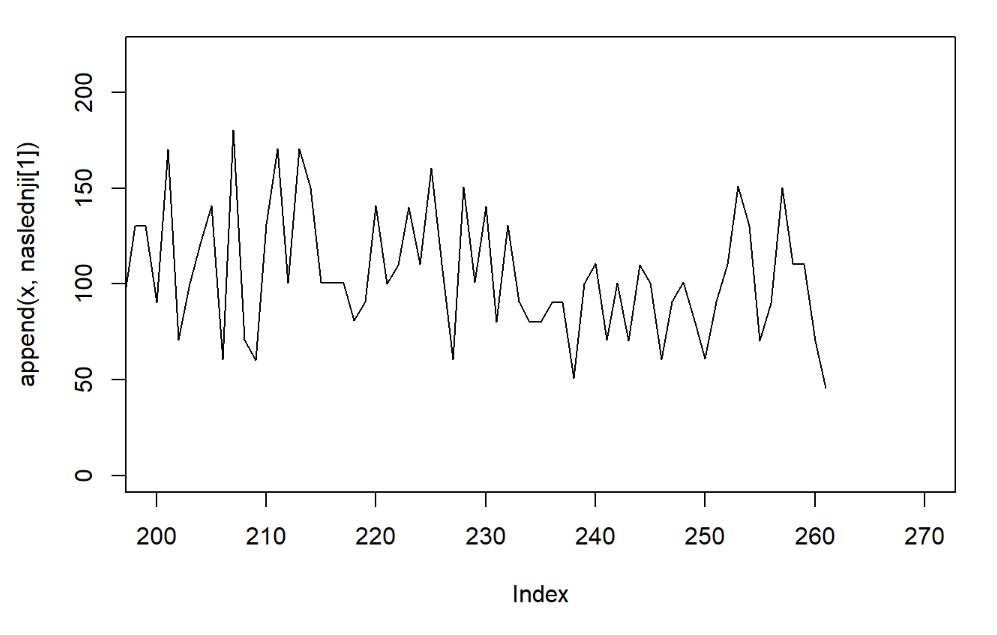
\includegraphics[width=1\textwidth]{naslednjiB.png}
\end{frame}

\begin{frame}
\centering Hvala za pozornost!
\end{frame}
\end{document}